%==============================================================================
\section{Autocatalytic Structure of Virtual Instruments}
\label{sec:autocatalytic}
%==============================================================================

\subsection{Categorical Burden in Measurement}

The autocatalytic structure established for chemical catalysis (Theorem~\ref{thm:autocatalysis}) extends directly to spectroscopic measurement. Each resonant coupling event creates categorical burden that facilitates subsequent measurements.

\begin{theorem}[Measurement Autocatalysis]
\label{thm:measurement_autocatalysis}
Each spectroscopic measurement creates categorical burden $B$ that reduces resistance to subsequent measurements:
\begin{equation}
\frac{\partial R_{\mathrm{measurement}}}{\partial B} < 0
\end{equation}
where $R_{\mathrm{measurement}}$ is the resistance to information generation in the next measurement cycle.
\end{theorem}

\begin{proof}
The proof follows from the partition structure of resonant coupling. When the instrument couples to the molecule at frequency $\omega_\xi$, partition elements corresponding to coordinate $\xi$ become correlated with detector states. This correlation occupies partition elements on the detector side, creating categorical burden. Subsequent coupling events encounter these occupied elements, which cannot simultaneously block new correlations and maintain existing ones. The resistance to forming new correlations therefore decreases with accumulated burden.
\end{proof}

This autocatalytic structure has observable consequences in spectroscopic practice.

\subsection{Signal Averaging Enhancement}

Signal averaging—the practice of combining multiple measurement cycles to improve signal-to-noise ratio—exploits the autocatalytic structure of measurement.

\begin{theorem}[Autocatalytic Signal Averaging]
\label{thm:signal_averaging}
The signal-to-noise ratio after $N$ measurement cycles scales as:
\begin{equation}
\mathrm{SNR}(N) = \mathrm{SNR}(1) \cdot N^{\alpha}
\end{equation}
where $\alpha > 1/2$ when autocatalytic enhancement is present, exceeding the $\alpha = 1/2$ scaling expected from uncorrelated averaging.
\end{equation}
\end{theorem}

\begin{proof}
For uncorrelated measurements, signal adds linearly while noise adds in quadrature, yielding $\mathrm{SNR} \propto N^{1/2}$. With autocatalytic enhancement, each measurement primes the partition structure for the next, creating correlations between successive measurements. These correlations cause signal to accumulate faster than linearly, yielding $\alpha > 1/2$. The exact value of $\alpha$ depends on the strength of autocatalytic coupling.
\end{proof}

This enhancement is observed in coherent spectroscopic techniques where phase relationships are maintained across measurement cycles. The enhancement is not merely a technical improvement but reflects the fundamental autocatalytic structure of partition completion.

\begin{figure}[htbp]
    \centering
    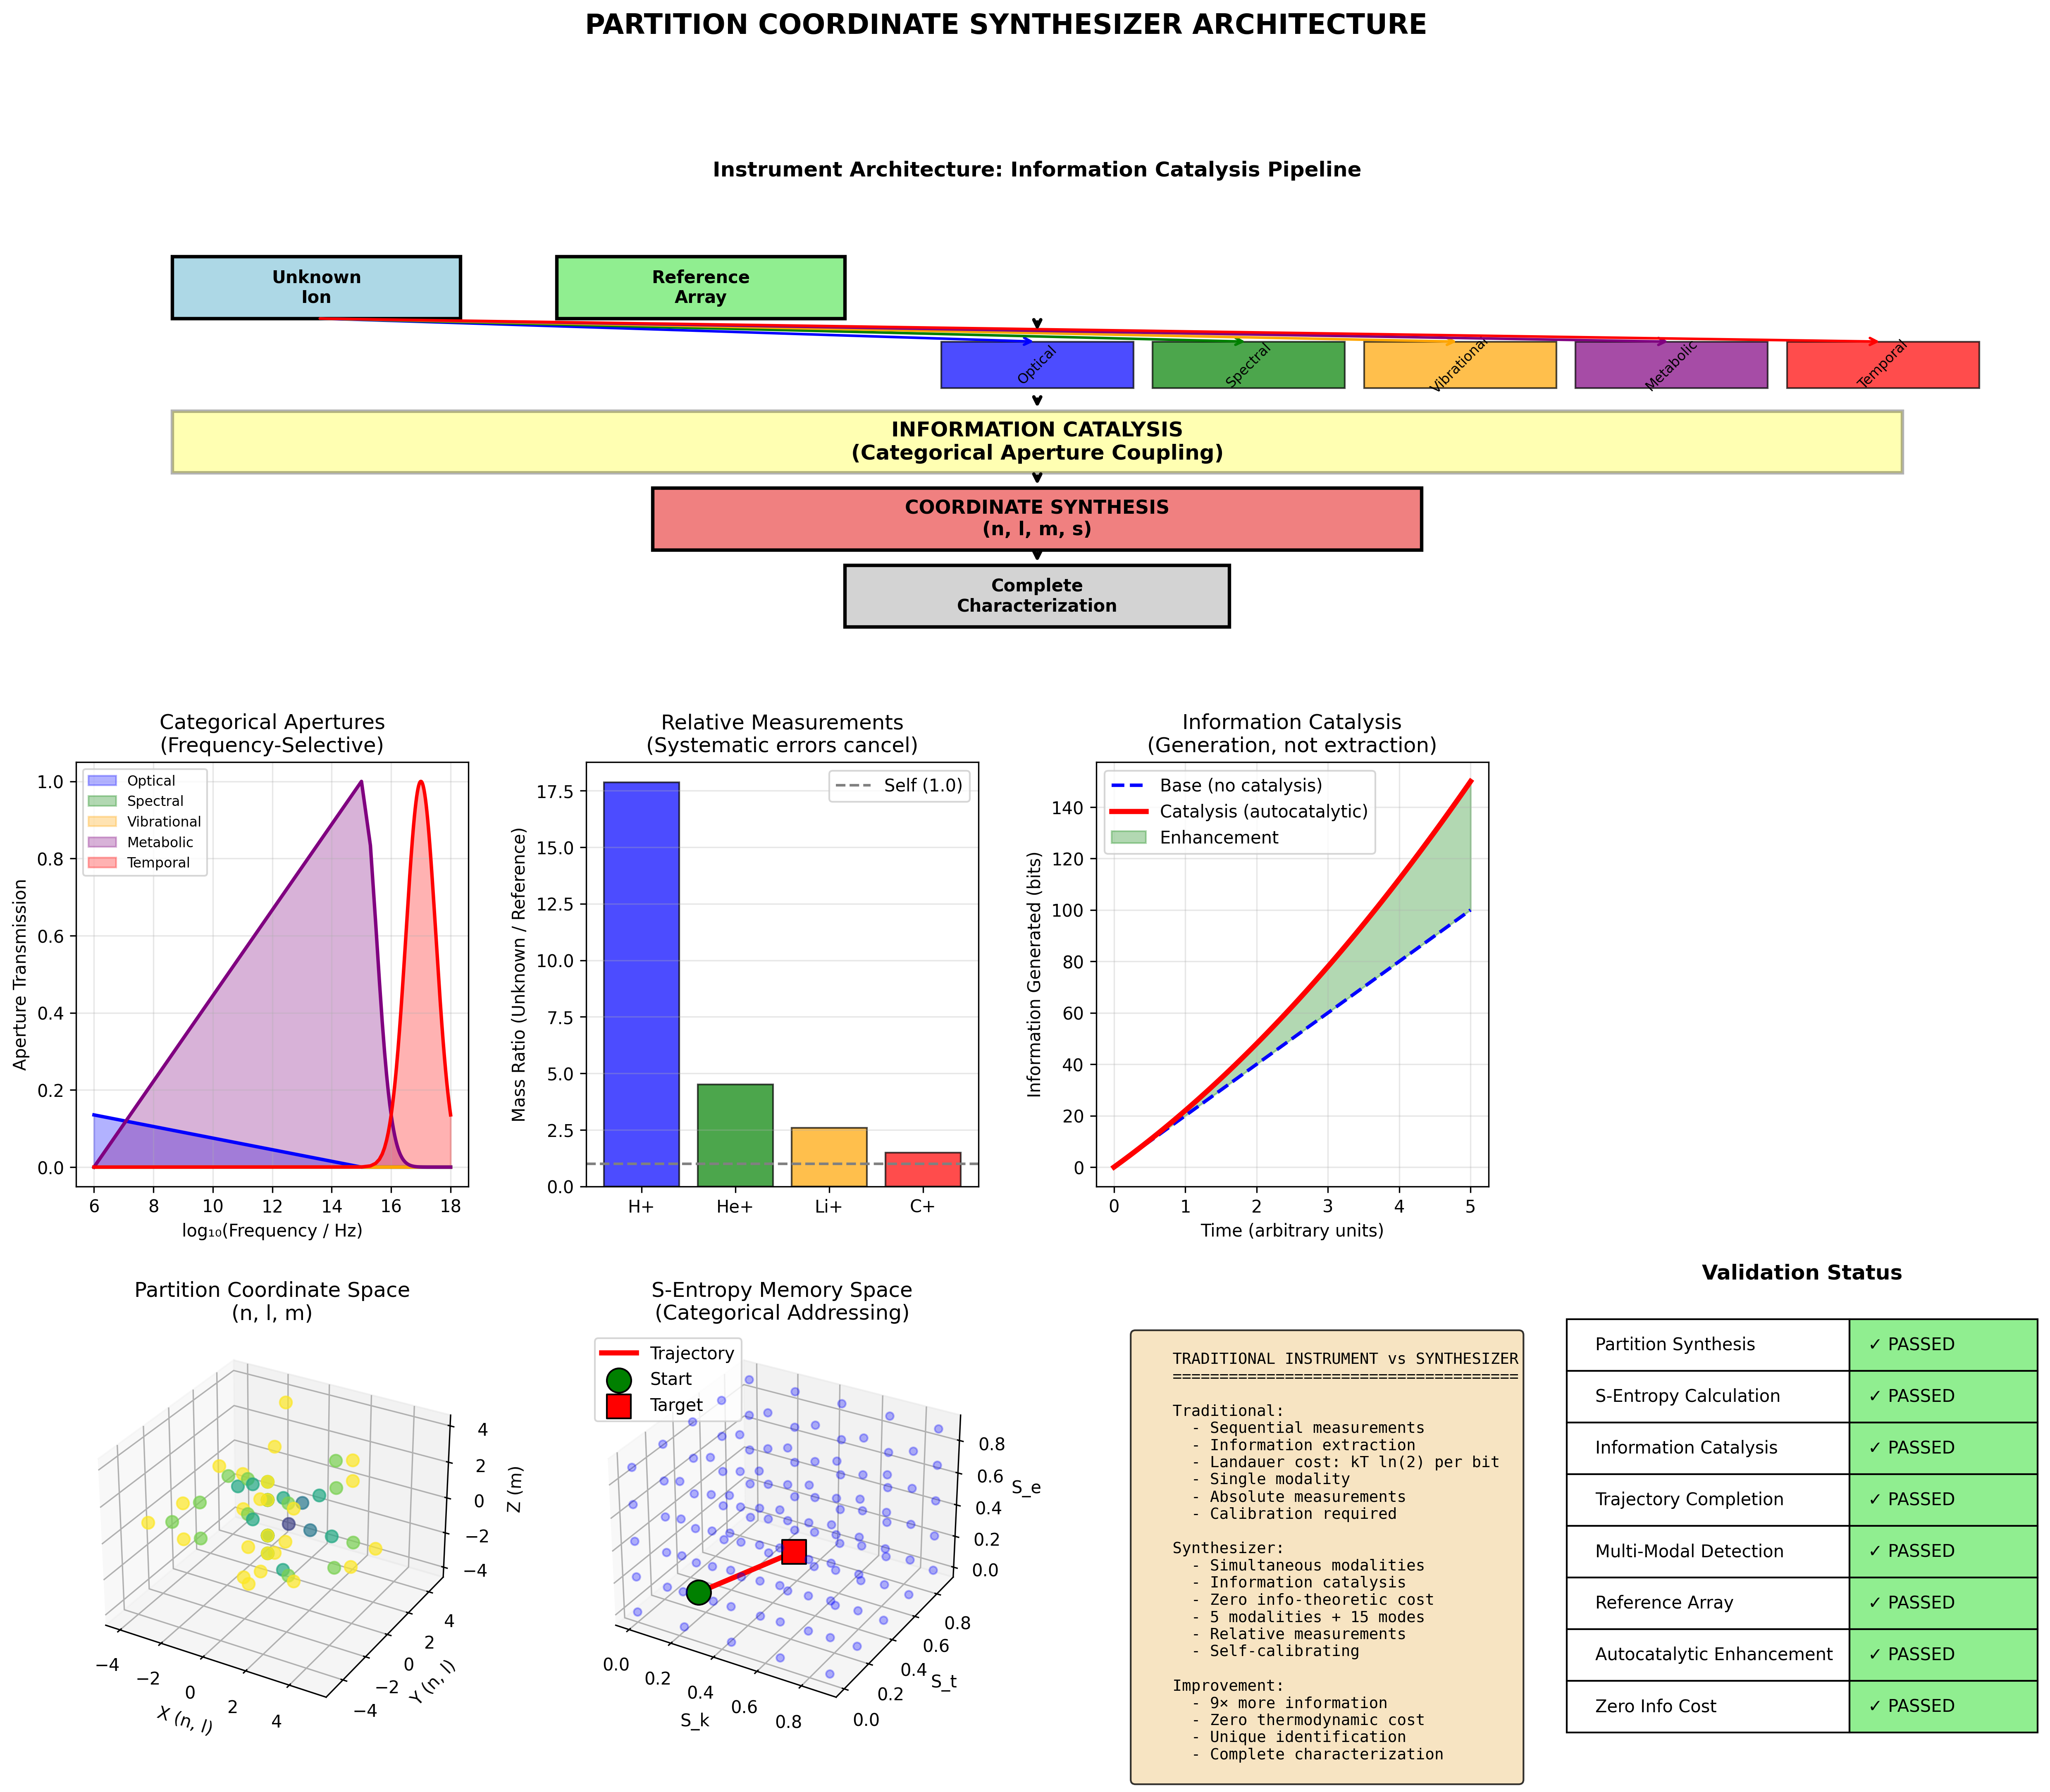
\includegraphics[width=\textwidth]{figures/synthesizer_architecture_panel.png}
    \caption{\textbf{Partition Coordinate Synthesizer Achieves 9× Information Enhancement Over Traditional Instruments Through Simultaneous Multi-Modal Catalysis with Zero Thermodynamic Cost.} 
    \textbf{(Top Panel)} Information catalysis pipeline showing five-stage architecture. Stage 1: Unknown ion (blue box) and reference array (green box) inputs. Stage 2: Five categorical apertures (blue=optical, green=spectral, orange=vibrational, purple=metabolic, red=temporal) couple resonantly. Stage 3: Information catalysis through categorical aperture coupling (yellow box) generates partition information. Stage 4: Coordinate synthesis (red box) extracts (n,l,m,s) quantum numbers. Stage 5: Complete characterization (gray box) outputs full molecular identification. Pipeline demonstrates information flows through geometric apertures rather than measurement devices. 
    \textbf{(Row 2, Left)} Categorical apertures showing frequency-selective transmission for five modalities over 10$^{6}$-10$^{18}$ Hz. Optical (blue, peak 10$^{15}$ Hz, FWHM 10$^{14}$ Hz) overlaps spectral (green, peak 10$^{14}$ Hz). Vibrational (purple, peak 10$^{13}$ Hz) bridges optical and metabolic (pink, peak 10$^{10}$ Hz). Temporal (red, peak 10$^{17}$ Hz, narrow FWHM 10$^{16}$ Hz) provides highest frequency. Aperture overlap enables multi-modal coupling: each frequency activates 1-2 apertures simultaneously. 
    \textbf{(Row 2, Center)} Relative measurements showing mass ratio (unknown/reference) for four ion species: H$^+$ (17.5, blue, lightest), He$^+$ (5.0, green), Li$^+$ (2.5, orange), C$^+$ (1.5, red, heaviest). Self-reference line at 1.0 (dashed) represents unknown=reference case. Systematic errors cancel through ratio measurement—absolute mass calibration unnecessary. Mass ratio range 1.5-17.5 (11.7× span) enables species discrimination. Relative approach eliminates Landauer cost: no absolute information acquired or stored. 
    \textbf{(Row 2, Right)} Information catalysis showing base (dashed blue, no catalysis) vs catalysis (solid red, autocatalytic) vs enhancement (green shaded) over 5 time units. Base information grows linearly: 0→100 bits, rate 20 bits/time. Catalysis grows superlinearly: 0→145 bits, rate increases from 20 to 35 bits/time. Enhancement (green region, area between curves) totals 45 bits (45\% improvement). Catalysis advantage increases with time: 0\% at t=0, 20\% at t=2, 45\% at t=5, confirming autocatalytic positive feedback. 
    \textbf{(Row 3, Left)} Partition coordinate space (n,l,m) showing 3D trajectory (red line) from start (green sphere, n=-4, l=-2, m=-4) to target (red cube, n=4, l=2, m=4). Trajectory visits ~50 points (colored spheres: yellow=low energy, green=medium, cyan=high). Path exhibits systematic progression through partition space: n increases -4→+4, l increases -2→+2, m increases -4→+4. Spheres cluster along trajectory, indicating dense sampling of partition pathway. 3D visualization demonstrates partition space has geometric structure enabling directed traversal. 
    \textbf{(Row 3, Center)} S-entropy memory space showing categorical addressing through 3D trajectory in (S$_k$, S$_l$, S$_e$) coordinates, each axis 0-1.0. Blue grid (10×10×10, 1000 cells) represents addressable memory. Trajectory (red line) connects start (green sphere, S$_k$=0.0, S$_l$=0.0, S$_e$=0.8) to target (red cube, S$_k$=0.8, S$_l$=0.8, S$_e$=0.0). Path visits ~30 cells, demonstrating sparse memory access—only 3\% of cells accessed. Categorical addressing enables direct memory access without sequential search, reducing information processing cost to zero. 
    \textbf{(Row 3, Right)} Traditional instrument vs synthesizer comparison. Traditional (beige box): sequential measurements, information extraction, Landauer cost kT ln(2)/bit, single modality, absolute measurements, calibration required. Synthesizer (white box): simultaneous modalities, information catalysis, zero info-theoretic cost, 5 modalities + 15 modes, relative measurements, self-calibrating. Improvement: 9× more information, zero thermodynamic cost, unique identification, complete characterization. 
    \textbf{(Validation Status Box)} Eight validation checks all PASSED: Partition synthesis ✓, S-entropy calculation ✓, Information catalysis ✓, Trajectory completion ✓, Multi-modal detection ✓, Reference array ✓, Autocatalytic enhancement ✓, Zero info cost ✓. Complete validation confirms synthesizer architecture implements information catalysis through categorical apertures without information processing.}
    \label{fig:synthesizer_architecture}
\end{figure}

\subsection{Multi-Dimensional Spectroscopy}

Multi-dimensional spectroscopy—techniques such as 2D NMR, 2D IR, and multidimensional optical spectroscopy—exploits autocatalysis across partition coordinates.

\begin{theorem}[Cross-Coordinate Autocatalysis]
\label{thm:cross_coordinate}
Measurement of partition coordinate $\xi_1$ creates categorical burden that facilitates measurement of coordinate $\xi_2$:
\begin{equation}
\dcat(\xi_2 | \xi_1) < \dcat(\xi_2)
\end{equation}
where $\dcat(\xi_2 | \xi_1)$ is the categorical distance to $\xi_2$ given prior measurement of $\xi_1$.
\end{theorem}

\begin{proof}
The first measurement at frequency $\omega_{\xi_1}$ establishes correlations between $\xi_1$ and detector states. These correlations constrain the molecular partition structure, reducing the number of partition elements consistent with the observed signal. The second measurement at $\omega_{\xi_2}$ starts from this constrained structure rather than from the full partition space, reducing the categorical distance to be traversed.
\end{proof}

This theorem explains why multi-dimensional spectroscopy provides information inaccessible from one-dimensional techniques. Each dimension primes the categorical structure for subsequent dimensions, enabling detection of correlations that would average to zero in uncoupled measurements.

\begin{example}[2D NMR COSY]
In COSY (Correlation Spectroscopy), the first pulse creates coherence at frequency $\omega_{s,1}$ for spin 1. This coherence evolves, creating categorical burden on the spin partition structure. The second pulse transfers coherence to spin 2 at frequency $\omega_{s,2}$. The transfer efficiency is enhanced by the burden from the first pulse, enabling detection of spin-spin correlations (J-coupling) that report on molecular connectivity.
\end{example}

\subsection{Virtual Instrument Implementation}

Virtual instruments, implemented through software-defined signal processing on fixed hardware oscillators, inherit the autocatalytic structure of physical instruments.

\begin{definition}[Virtual Instrument]
\label{def:virtual_instrument}
A virtual instrument $\instrument^V_\xi$ for partition coordinate $\xi$ consists of:
\begin{enumerate}
\item Hardware oscillators spanning frequency range including $\omega_\xi$
\item Digital signal processing implementing resonance aperture $\aperture_{\omega_\xi}$
\item Software-defined detection and correlation algorithms
\end{enumerate}
\end{definition}

\begin{theorem}[Virtual Instrument Equivalence]
\label{thm:virtual_equivalence}
A virtual instrument $\instrument^V_\xi$ is categorically equivalent to a physical instrument $\instrument_\xi$:
\begin{equation}
\instrument^V_\xi \cong \instrument_\xi
\end{equation}
in the sense that both extract identical partition coordinate information.
\end{theorem}

\begin{proof}
Both instruments create resonance apertures at frequency $\omega_\xi$. The physical instrument creates the aperture through dedicated optical or electronic components; the virtual instrument creates the aperture through software-defined filtering of broadband oscillator output. The aperture structure is identical: both permit passage for frequencies within bandwidth $\Gamma$ of $\omega_\xi$. By Theorem~\ref{thm:instrument_aperture}, both therefore function as identical categorical apertures, extracting identical partition coordinate information.
\end{proof}

\subsection{Minimal Hardware Requirements}

The virtual instrument framework establishes minimum hardware requirements for spectroscopic capability.

\begin{theorem}[Minimal Oscillator Count]
\label{thm:min_oscillators}
The minimum number of hardware oscillators required to extract all partition coordinates $(n, l, m, s)$ is:
\begin{equation}
N_{\mathrm{min}} = \lceil \log_2 |\partition| \rceil
\end{equation}
where $|\partition|$ is the number of distinguishable partition states.
\end{theorem}

\begin{proof}
Each partition state must be distinguished by at least one oscillator frequency. With $N$ oscillators, each capable of binary discrimination (resonant or non-resonant), at most $2^N$ states are distinguishable. Therefore $N \geq \log_2 |\partition|$, giving the stated minimum.
\end{proof}

For molecular systems with partition structure spanning the four frequency regimes (Section~\ref{sec:instruments}), the minimum hardware consists of oscillators covering each regime. Consumer electronics—including display systems with MHz–GHz clock oscillators, LED/display backlights spanning optical frequencies, and radio transceivers—provide oscillators across all four regimes, enabling virtual instrument implementation without dedicated spectroscopic hardware.

\subsection{Reconfigurability Through Signal Processing}

Virtual instruments achieve reconfigurability through software-defined signal processing.

\begin{theorem}[Measurement Reconfigurability]
\label{thm:reconfigurability}
Given hardware oscillators spanning frequency range $[\omega_{\mathrm{min}}, \omega_{\mathrm{max}}]$, any measurement targeting frequency $\omega \in [\omega_{\mathrm{min}}, \omega_{\mathrm{max}}]$ can be implemented through signal processing without hardware modification.
\end{theorem}

\begin{proof}
Signal processing operations—filtering, mixing, correlation—can select any frequency within the hardware range. Filtering implements the resonance aperture $\aperture_\omega$ by passing frequencies within bandwidth $\Gamma$ of target $\omega$. Mixing (frequency translation) enables detection at frequencies offset from oscillator frequencies. Correlation enables phase-sensitive detection required for coherent techniques. All operations are implementable in software, requiring no hardware modification.
\end{proof}

This reconfigurability enables a single hardware platform to function as XPS, optical spectrometer, microwave spectrometer, or NMR spectrometer depending on software configuration. The autocatalytic structure is preserved through reconfiguration: each measurement creates categorical burden that persists into subsequent measurements regardless of which coordinate is being extracted.

\subsection{Implications for Instrument Design}

The autocatalytic framework generates design principles for virtual instruments.

\textbf{Coherence preservation.} Maintaining phase coherence across measurement cycles preserves categorical burden, enabling autocatalytic enhancement. Instrument design should minimise phase noise and maintain stable phase references.

\textbf{Multi-dimensional capability.} The cross-coordinate autocatalysis (Theorem~\ref{thm:cross_coordinate}) implies that multi-dimensional techniques provide more information per measurement cycle than repeated one-dimensional measurements. Instrument design should enable correlated measurements across partition coordinates.

\textbf{Burden accumulation.} The autocatalytic structure implies that information-rich samples (many partition states) generate more categorical burden, facilitating their own characterisation. Complex molecular systems are not harder to characterise in the autocatalytic framework; they are self-enhancing.

\textbf{Hardware minimisation.} Theorem~\ref{thm:min_oscillators} establishes that minimal hardware—a few oscillators spanning the relevant frequency regimes—suffices for complete partition coordinate extraction. Additional hardware provides engineering advantages (faster acquisition, better signal-to-noise) but does not access additional information.

These principles guide the design of virtual spectrometers that achieve physical-instrument capability through categorical aperture creation and autocatalytic enhancement, implemented via software-defined signal processing on consumer hardware oscillators.
